\section{Results}
\subsection{Dominant wind with random noise}
In order to find the maximum wind speed that complies with our definition of the problem in Section2.2.1, wind patterns with different speed distributions were tested in our simulation environment. We aim to find the maximum wind speed that enables the quadcopter to stay around the target within 20 cm for 30 s. For this reason, the simulation for each wind model is suspended once the distance from the origin reaches 20cm. $t_20$ for each wind model is obtained as the average of 10 simulations under the same condition. The simulation data is summarized in Table\ref{tab: sim}.

Referring from the table, we can roughly find the maximum wind speed $v_M = 5$ m/s.

 \begin{table}[H] 
 \centering 
 \begin{tabular}{|c|c|c|}
 \hline
 Wind Speed [m/s]& Deviation of the Wind Speed [m/s]&  $t_{20}$ [s] \\ \hline \hline
   2  & 0.01  & 45.55 \\ \hline
 2  & 0.11  & 36.59\\ \hline
 2  & 0.21 & 28.27\\ \hline
 2  & 0.31  & 23.58\\ \hline
 2  & 0.41  & 22.11 \\ \hline
 2  & 0.51  & 18.79\\ \hline
 2  & 0.61  & 12.10\\ \hline
 3  & 0.01  & 48.70\\ \hline
 3  & 0.11  & 35.68\\ \hline
 3  & 0.21  & 31.36\\ \hline
 3  & 0.31  & 15.73\\ \hline
 3  & 0.41  & 17.83\\ \hline
 3  & 0.51  & 15.02\\ \hline
 3  & 0.61  & 12.75\\ \hline
 4  & 0.01  & 53.68\\ \hline
 4  & 0.11  & 45.48\\ \hline
 4  & 0.21  & 30.09\\ \hline
 4  & 0.31  & 20.69\\ \hline
 4  & 0.41 & 16.35\\ \hline
 4  & 0.51  & 14.25\\ \hline
 4  & 0.61  & 12.85\\ \hline
 5  & 0.01  & 54.13\\ \hline
 5  & 0.11  & 54.89\\ \hline
 5  & 0.21  & 45.45\\ \hline
 5  & 0.31  & 15.63\\ \hline
 5  & 0.41 & 23.66\\ \hline
 5  & 0.51  & 13.81\\ \hline
 5  & 0.61  & 10.56\\ \hline
 6  & 0.01  & 60.59\\ \hline
 6  & 0.11  & 53.93\\ \hline
 6  & 0.21  & 26.38\\ \hline
 6  & 0.31  & 21.37\\ \hline
 6  & 0.41 & 19.43\\ \hline
 6  & 0.51  & 10.83\\ \hline
 6  & 0.61  & 8.41\\ \hline
 7  & 0.01  & 42.67\\ \hline
 7  & 0.11  & 28.90\\ \hline
 7  & 0.21  & 34.13\\ \hline
 7  & 0.31  & 21.08\\ \hline
 7  & 0.41  & 20.81\\ \hline
 7  & 0.51  & 13.50\\ \hline
 7  & 0.61  & 9.95\\ \hline
 \end{tabular}% 
 \caption{Simulation Data} 
 \label{tab: sim}% 
 \end{table}% 
To make our simulation more convincing, four sample simulation trajectories are plotted in Figure \ref{fig: traj}. Each subfigure was simulated under wind speed of 5 m/s and deviation of 0.1m/s. The trajectories consist of positions of center of mass during the simulations. These plots demonstrate how the control system manages to keep the quadcopter near the origin when it's subject to the wind. 

The wind field is also visualized in Figure \ref{fig: wind} to give an clear intuition of how it varies in direction and magnitude through time. The dataset of wind speed in the figure has deviation of 0.2 m/s. Each line represents the wind speed at an instant. The color of the end point of the lines vary continuously from deep brown to pale yellow.

\begin{figure}[H]
\begin{subfigure}{.5\textwidth}
\centering
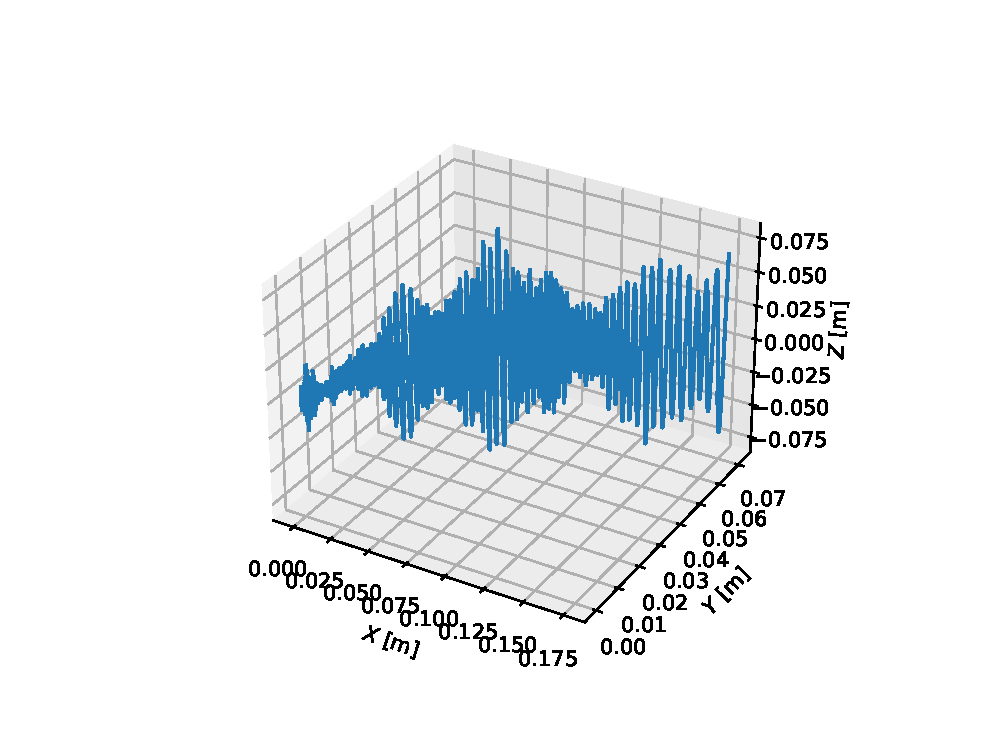
\includegraphics[width=\linewidth]{Images/trajectory 1.eps}
\caption{Trajectory 1}
\end{subfigure}
\hfill
\begin{subfigure}{.5\textwidth}
\centering
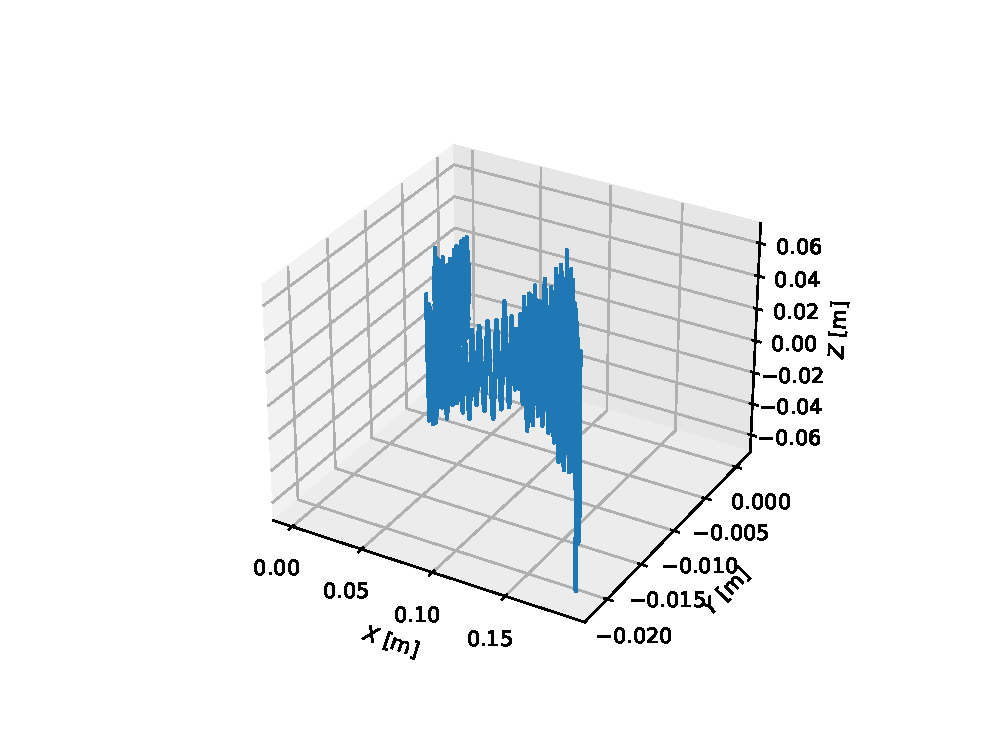
\includegraphics[width=\linewidth]{Images/trajectory 2.eps}
\caption{Trajectory 2}
\end{subfigure}
\hfill
\begin{subfigure}{.5\textwidth}
\centering
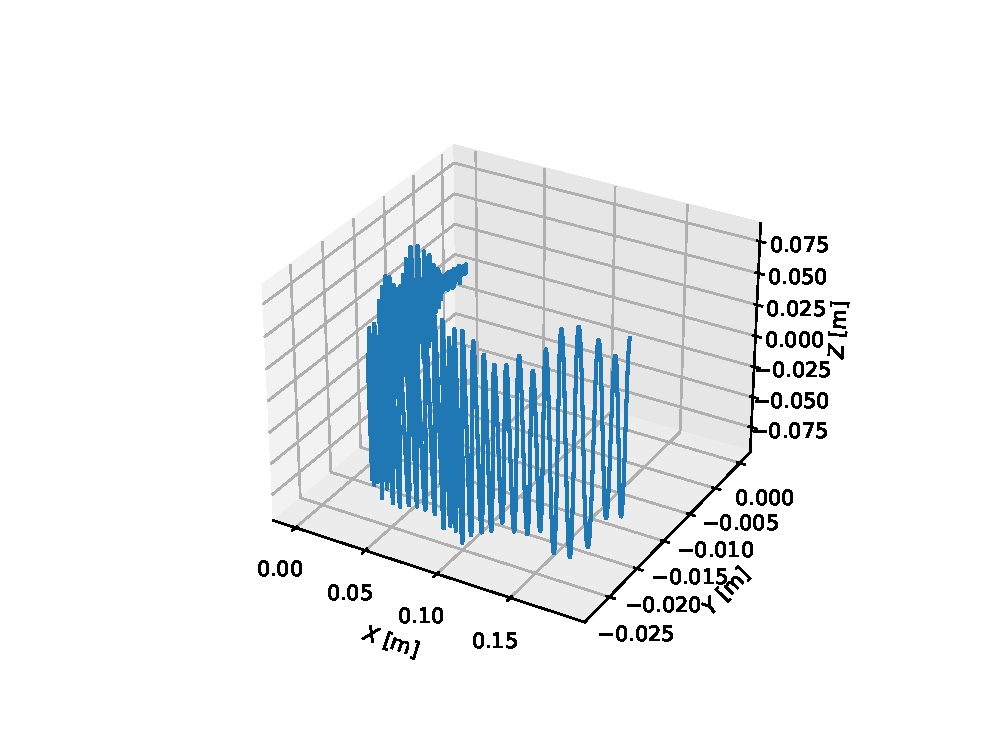
\includegraphics[width=\linewidth]{Images/trajectory 3.eps}
\caption{Trajectory 3}
\end{subfigure}
\begin{subfigure}{.5\textwidth}
\centering

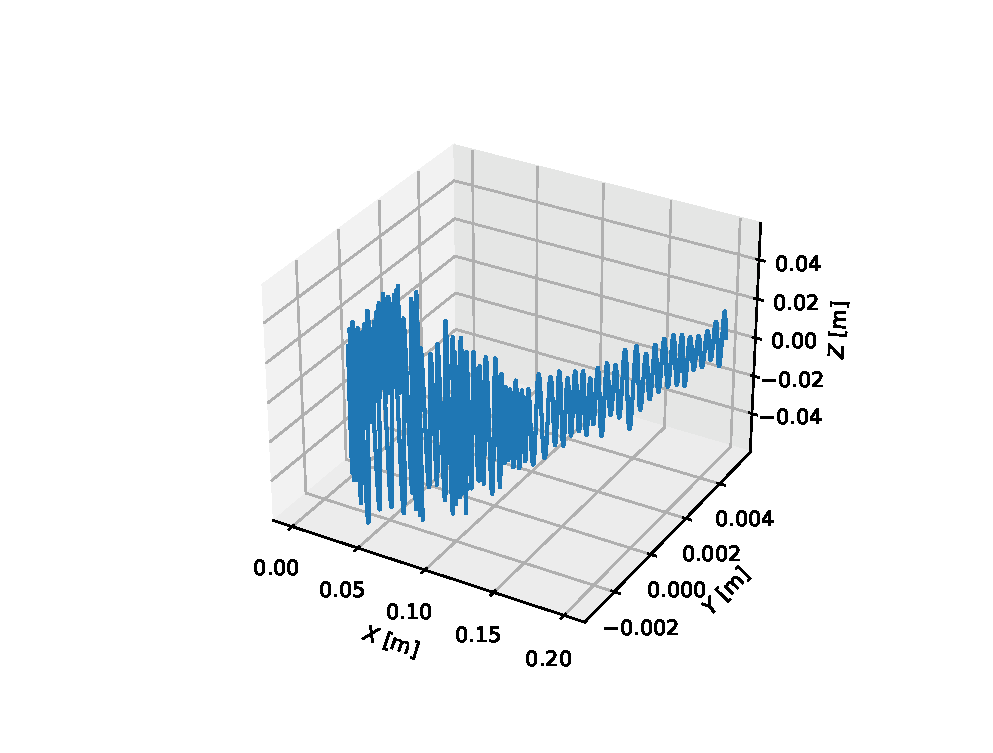
\includegraphics[width=\linewidth]{Images/trajectory 4.eps}
\caption{Trajectory 4}
\end{subfigure}
\caption{Sample Trajectories for Wind Speed = 5 m/s}
\label{fig: traj}
\end{figure}

\begin{figure}[H]
    \centering
    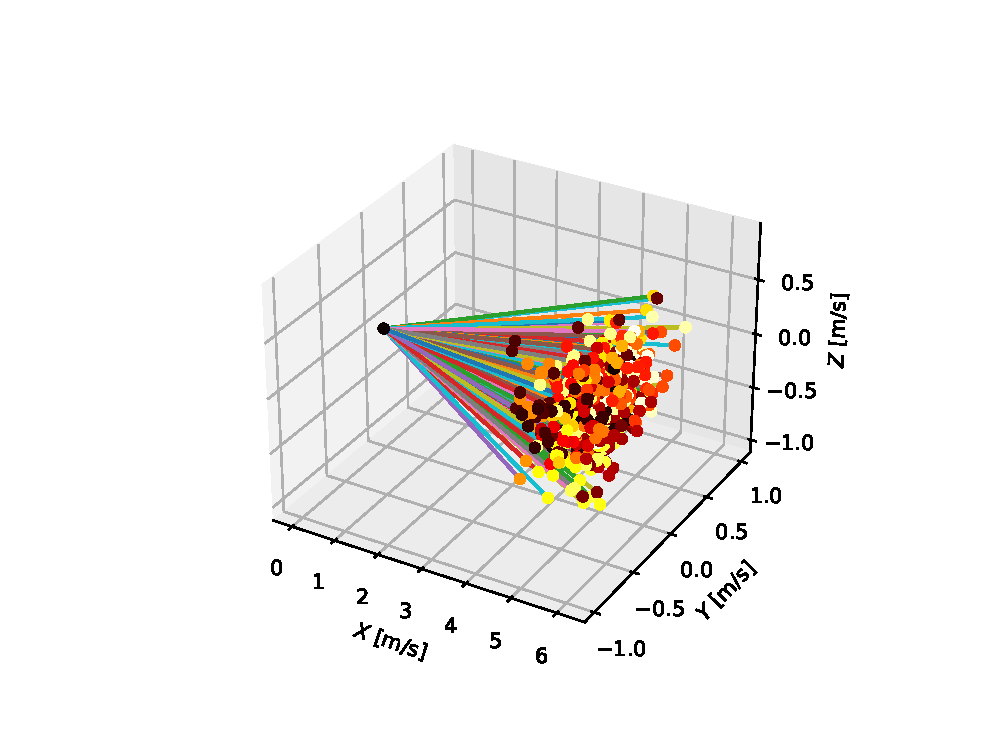
\includegraphics[width=.8\linewidth]{Images/wind.eps}
    \caption{Visualization of Wind}
    \label{fig: wind}
\end{figure}



\subsection{Periodic wind}
From Fourier analysis we know that any periodical wind can be decomposed into a series of wind with sinusoidal velocity components. Figure \ref{fig: windSin} exhibits the possible wind speed with sinusoidal velocity components.

Therefore the study of periodical wind with sinusoidal velocity components is crucial as it can help us predicate the behavior of the quadcopter under more general periodical wind patterns.
In this section we observe periodic wind with sinusoidal velocity component in the x-axis direction.
In order to find the maximum wind speed that complies with our definition of the problem in Section2.2.1, wind with different amplitude and frequency were tested in our simulation environment. Again, $t_20$ denotes the time at which the distance from the origin reaches 20cm. The simulation data is summarized in Table\ref{tab: simSin} and Table\ref{tab:simSin2}.

Referring from the table, we can conclude that our control model cannot handle wind with varying magnitude as perfectly as it does with dominant wind patterns. With fixed amplitude, the stability becomes worse at the frequency of the change of wind's velocity increases. However, we can also notice that the stability is less sensitive to increasement of frequency at lower amplitudes.

Under frequency $f = 0.01$ Hz, the performance reaches our expectation only when the amplitude of the velocity of wind is no larger than $0.95$ m/s. When the frequency becomes larger, the quadcopter will be able to keep itself stable under lower amplitudes.

For periodic wind, four sample simulation trajectories are plotted in Figure \ref{fig: trajSin}. Each subfigure was simulated under amplitude $1.2$m and frequency $0.01$ Hz. The trajectories consist of positions of center of mass during the simulations. These plots demonstrate how the control system manages to keep the quadcopter near the origin when it's subject to periodical wind.



\begin{figure}[H]
\begin{subfigure}{.5\textwidth}
\centering
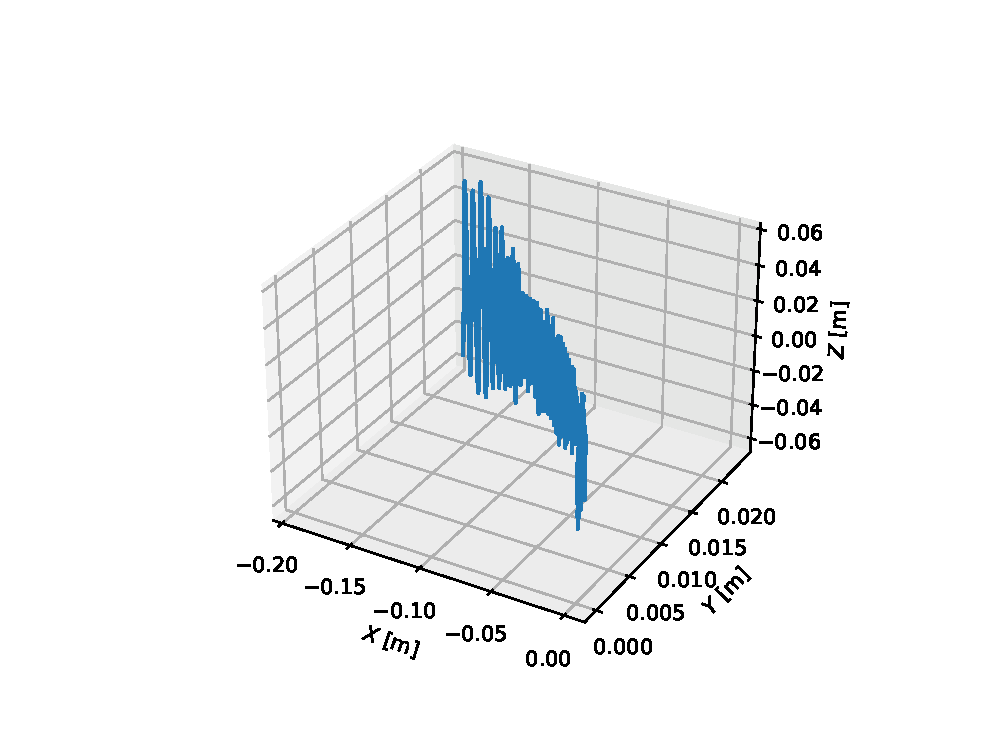
\includegraphics[width=\linewidth]{Images/trajectory_sin.eps}
\caption{Trajectory 1}
\end{subfigure}
\hfill
\begin{subfigure}{.5\textwidth}
\centering
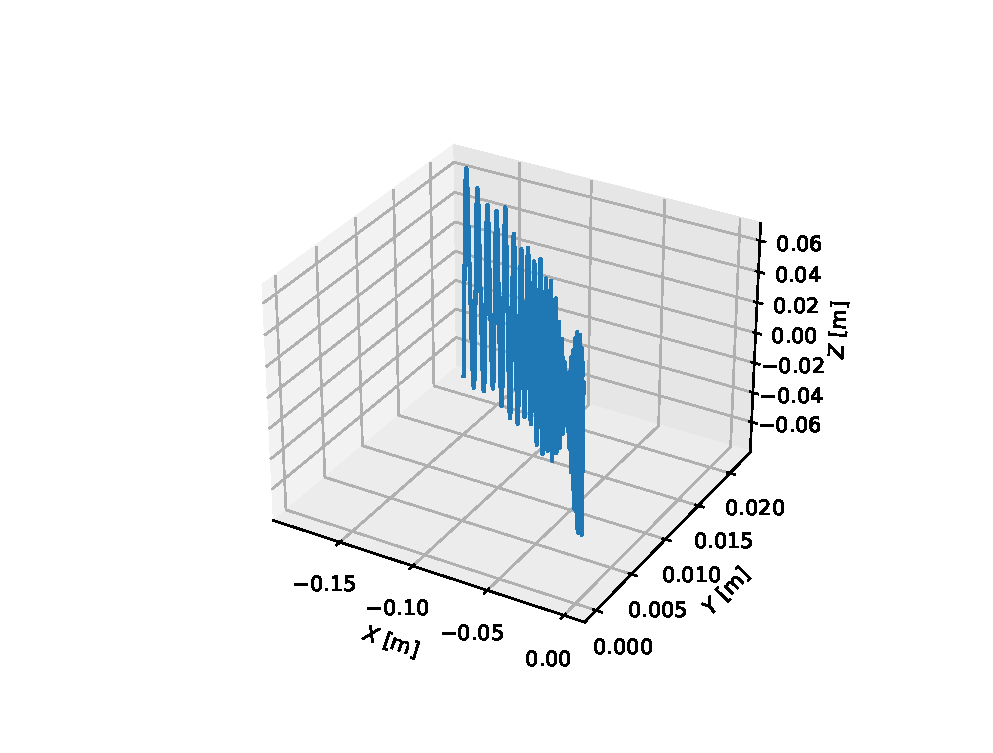
\includegraphics[width=\linewidth]{Images/trajectory_sin copy.eps}
\caption{Trajectory 2}
\end{subfigure}
\hfill
\begin{subfigure}{.5\textwidth}
\centering
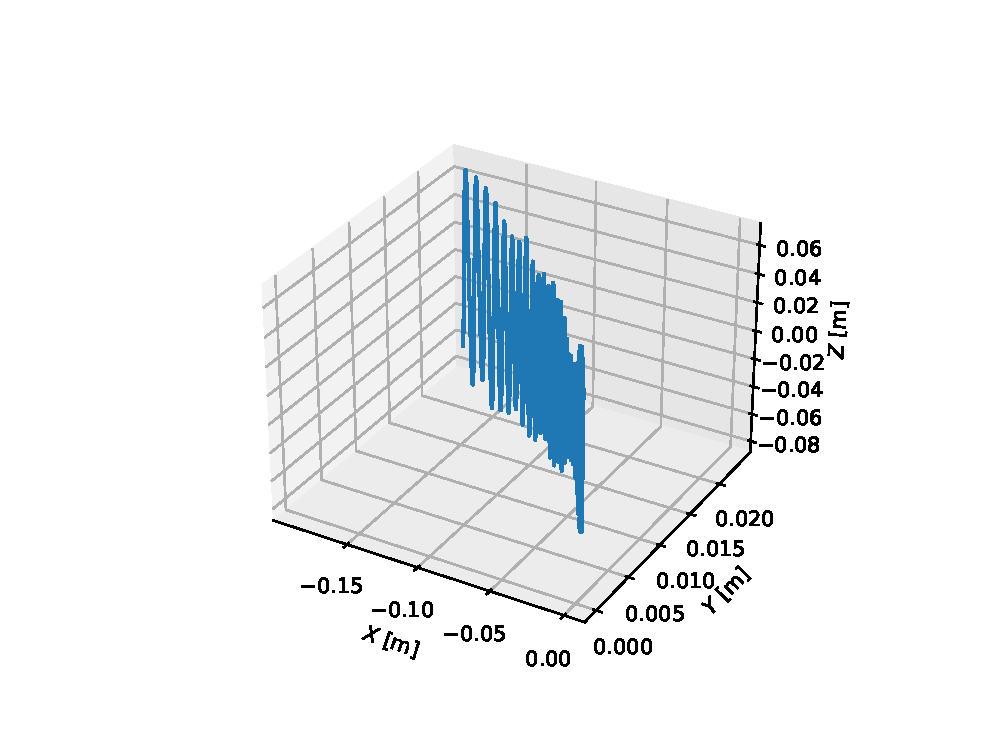
\includegraphics[width=\linewidth]{Images/trajectory_sin copy 2.eps}
\caption{Trajectory 3}
\end{subfigure}
\begin{subfigure}{.5\textwidth}
\centering

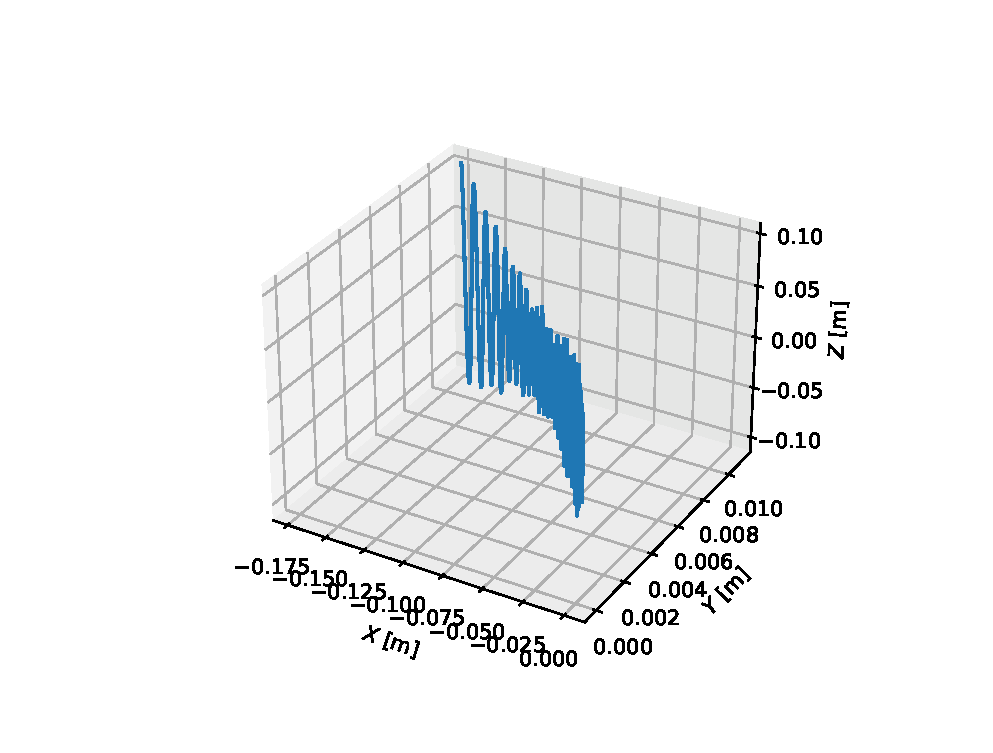
\includegraphics[width=\linewidth]{Images/trajectory_sin copy 3.eps}
\caption{Trajectory 4}
\end{subfigure}
\caption{Sample Trajectories for Wind Speed = 5 m/s}
\label{fig: trajSin}
\end{figure}

\begin{figure}[H]
    \centering
    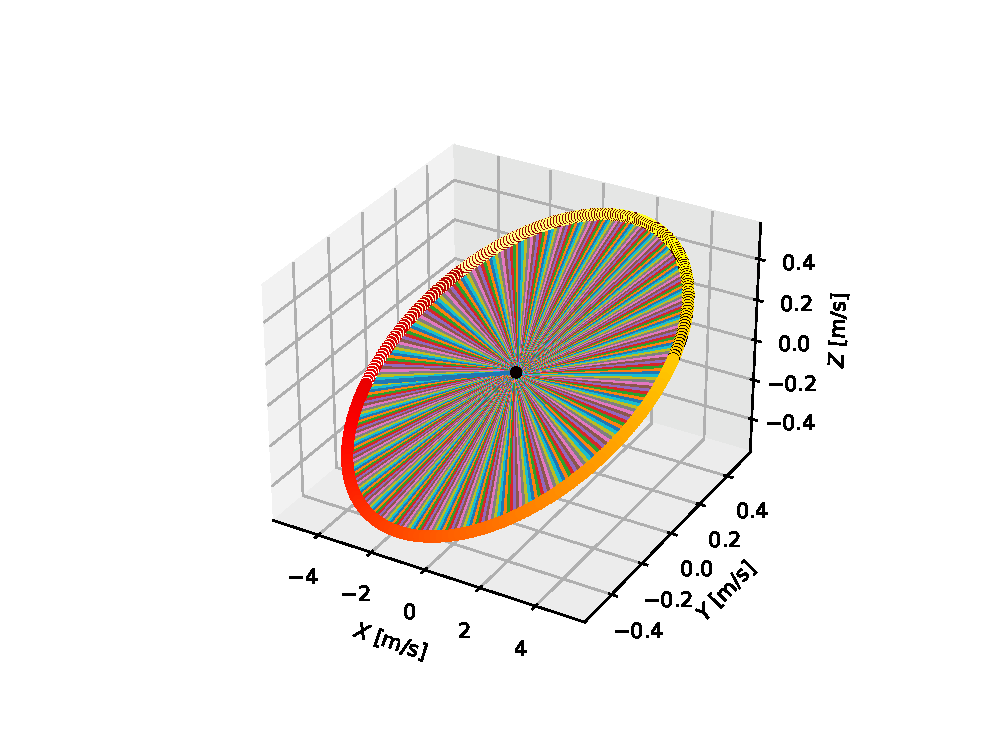
\includegraphics[width=.8\linewidth]{Images/wind_sin.eps}
    \caption{Visualization of Wind}
    \label{fig: windSin}
\end{figure}




 \begin{table}[H] 
 \centering 
 \begin{tabular}{|c|c|c|}
 \hline
 Speed Amplitude [m/s] & frequency [Hz] & $t_{20}$ [s] \\ \hline


1.001 & 0.01 & 26.54 \\ \hline
1.001 & 0.02 & 20.50 \\ \hline
1.001 & 0.03 & 18.08 \\ \hline
1.001 & 0.04 & 16.60\\ \hline
1.001 & 0.05 & 15.78 \\ \hline
1.001 & 0.060 & 15.28 \\ \hline
1.001 & 0.070 & 15.27 \\ \hline
2.001 & 0.01 & 17.73 \\ \hline
2.001 & 0.02 & 13.45 \\ \hline
2.001 & 0.03 & 11.63 \\ \hline
2.001 & 0.04 & 10.53 \\ \hline
2.001 & 0.05 & 9.72 \\ \hline
2.001 & 0.060 & 9.12 \\ \hline
2.001 & 0.070 & 8.66 \\ \hline
3.001 & 0.01 & 14.66 \\ \hline
3.001 & 0.02 & 10.67 \\ \hline
3.001 & 0.03 & 8.99 \\ \hline
3.001 & 0.04 & 8.070\\ \hline
3.001 & 0.05 & 7.47 \\ \hline
3.001 & 0.060 & 7.00 \\ \hline
3.001 & 0.070 & 6.630\\ \hline



 \end{tabular}% 
 \caption{Periodic Wind Simulation Data Table 1} 
 \label{tab: simSin}% 
 \end{table}% 

 \begin{table}[H] 
 \centering 
 \begin{tabular}{|c|c|c|}
 \hline
 Speed Amplitude [m/s] & frequency [Hz] & $t_{20} [s]$ \\ \hline

 0.7 & 0.001 & 44.86 \\ \hline
0.7 & 0.011 & 32.46 \\ \hline
0.7 & 0.021 & 24.67 \\ \hline
0.7 & 0.031 & 21.93 \\ \hline
0.7 & 0.041 & 21.05 \\ \hline
0.7 & 0.051 & 21.05 \\ \hline
0.7 & 0.061 & 21.31 \\ \hline
0.75 & 0.001 & 44.58 \\ \hline
0.75 & 0.011 & 30.70 \\ \hline
0.75 & 0.021 & 24.09 \\ \hline
0.75 & 0.031 & 21.29 \\ \hline
0.75 & 0.041 & 20.19 \\ \hline
0.75 & 0.051 & 19.96 \\ \hline
0.75 & 0.061 & 20.20 \\ \hline
0.8 & 0.001 & 44.26 \\ \hline
0.8 & 0.011 & 30.09 \\ \hline
0.8 & 0.021 & 23.26 \\ \hline
0.8 & 0.031 & 20.24 \\ \hline
0.8 & 0.041 & 19.24 \\ \hline
0.8 & 0.051 & 18.76 \\ \hline
0.8 & 0.061 & 19.01 \\ \hline
0.85 & 0.001 & 47.57 \\ \hline
0.85 & 0.011 & 27.78 \\ \hline
0.85 & 0.021 & 21.95 \\ \hline
0.85 & 0.031 & 19.73 \\ \hline
0.85 & 0.041 & 18.33 \\ \hline
0.85 & 0.051 & 17.88 \\ \hline
0.85 & 0.061 & 17.89 \\ \hline
0.9 & 0.001 & 45.60 \\ \hline
0.9 & 0.011 & 27.46 \\ \hline
0.9 & 0.021 & 21.31 \\ \hline
0.9 & 0.031 & 19.03 \\ \hline
0.9 & 0.041 & 17.83 \\ \hline
0.9 & 0.051 & 17.12 \\ \hline
0.9 & 0.061 & 17.08 \\ \hline
0.95 & 0.001 & 47.43 \\ \hline
0.95 & 0.011 & 26.25 \\ \hline
0.95 & 0.021 & 20.77 \\ \hline
0.95 & 0.031 & 18.52 \\ \hline
0.95 & 0.041 & 17.11 \\ \hline
0.95 & 0.051 & 16.38 \\ \hline
0.95 & 0.061 & 16.00 \\ \hline



 \end{tabular}% 
 \caption{Periodic Wind Simulation Data Table 2} 
 \label{tab:simSin2}% 
 \end{table}% 








% \begin{itemize}

% \item Present the solution following from the model you have constructed.
% \item List ALL values of the numerical parameters you have used (you may do it in the caption of graphs/tables);
% \item All graphs, tables etc. appear in this part. They are used to illustrate how results depend on any parameters/initial conditions in the problem.  They should be clearly labeled.

% \item The error analysis is required if you report an experiment, also a numerical one. In our case it probably will not be needed.


% \begin{figure}[h]
% \begin{center}
% %\includegraphics[scale=0.5]{hm6_bar.eps}
% \caption{Put the figure's caption here. Give the values of all parameters ($a=1\ {\rm{m}}$, $C = 10^{-5}\ {\rm{kg}})$.  You may also do it directly in the graph.}
% \end{center}
% \end{figure}

% \item  Discuss the dependence of the results on the values of parameters. Highlight the trends, point out any unusual behavior/properties your model may display;


% \end{itemize}
